\documentclass[11pt,a4paper]{article}
\usepackage[utf8]{inputenc}
\usepackage[T1]{fontenc}
\usepackage[english]{babel}
\usepackage{amsmath}
\usepackage{amsfonts}
\usepackage{amssymb}
\usepackage{graphicx}
\usepackage{listings}
\usepackage{xcolor}
\usepackage{hyperref}

\definecolor{delim}{RGB}{20,105,176}
\definecolor{numb}{RGB}{106, 109, 32}
\definecolor{string}{rgb}{0.64,0.08,0.08}
\lstdefinelanguage{json}{
	numbers=left,
	numberstyle=\small,
	frame=single,
	rulecolor=\color{black},
	showspaces=false,
	showtabs=false,
	breaklines=true,
	postbreak=\raisebox{0ex}[0ex][0ex]{\ensuremath{\color{gray}\hookrightarrow\space}},
	breakatwhitespace=true,
	basicstyle=\ttfamily\small,
	upquote=true,
	morestring=[b]",
	stringstyle=\color{string},
	literate=
	*{0}{{{\color{numb}0}}}{1}
	{1}{{{\color{numb}1}}}{1}
	{2}{{{\color{numb}2}}}{1}
	{3}{{{\color{numb}3}}}{1}
	{4}{{{\color{numb}4}}}{1}
	{5}{{{\color{numb}5}}}{1}
	{6}{{{\color{numb}6}}}{1}
	{7}{{{\color{numb}7}}}{1}
	{8}{{{\color{numb}8}}}{1}
	{9}{{{\color{numb}9}}}{1}
	{\{}{{{\color{delim}{\{}}}}{1}
	{\}}{{{\color{delim}{\}}}}}{1}
	{[}{{{\color{delim}{[}}}}{1}
	{]}{{{\color{delim}{]}}}}{1},
}
\lstset{
	breaklines=true,
	tabsize=2,
	showstringspaces=false
}
\bibliographystyle{czechiso}

\author{Svätopluk Hanzel}
\title{Project proposal}

\begin{document}
\begin{titlepage}
	\begin{center}
		{\LARGE\textsc{Brno University of Technology}}\\
		\smallskip
		{\Large\textsc{Faculty of Information Technology}}\\
		\bigskip
		\vspace{\stretch{0.382}}
		\smallskip
		\huge{PDB}\\
		\huge{\textbf{Night snack}}\\
		\Large{Final report}
		\vspace{\stretch{0.618}}
	\end{center}
	{\today \hfill Svätopluk Hanzel}
\end{titlepage}

\section{Project overview}
	The goal of this project is to implement a simple system that can act as a demo of a food delivery company specialized in late-night deliveries for programmers.
	
	Since this is a demo application, the real-world usability is quite limited and this project mainly focuses on properly implementing CQRS and event sourcing patterns and using the correct DB systems for various types of data.
	
	\subsection{Application principle}\label{sec:app-principle}
		Main principle of the application can be described as follows: there are restaurants, which have menu items organized into categories, which can be ordered by customers. Since the menu items' price, customer's location and delivery status must be freezed in each order, the orders are saved separately with all the data in a single object.
		
		The main objective in this project was to optimize the application for scalability with regards to reads. The most common operation in such 

\section{Data}\label{sec:data}
	As described in Application principle (\ref{sec:app-principle}), the application works with \texttt{Restaurants}, \texttt{Menu categories}, \texttt{Menu items}, \texttt{Orders}.
	
	The first three are saved in CockroachDB for validation and administration purposes. These are read only by Command handlers. The Restaurant is then also saved in MongoDB along with its categories and items. This is done to optimize reads as more people would be browsing restaurant menus than updating them.
	
	\begin{figure}[h]
		\centering
		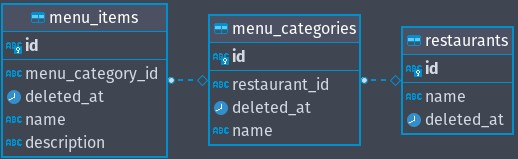
\includegraphics[width=0.7\linewidth]{img/er.jpg}
		\caption{Relations betweeen entities in CockroachDB}
		\label{fig:er}
	\end{figure}
	
	
	\subsection{MongoDB}
	MongoDB is used as NoSQL database to store Events, Restaurants, Stock and Orders. All of them are loaded from events to ensure consistency.
	
	\subsection{Data consistency}\label{sec:data-consistency}
		Since the data is distributed across various databases, the event sourcing pattern has been used. All commands generate events, which are saved into a persistent storage -- event store. All of these events are versioned. This ensures consistency since the aggregator cannot be updated if the updatee version doesn't correspond to the current version plus one.
	
\section{Architecture}
	The project in its current state consists of one main service -- \textit{Snacker}. Which further encapsulates these gRPC services:
	\begin{enumerate}
		\item SnackerService
		\item RestaurantCommandService
		\item RestaurantQueryService
		\item StockService
		\item OrderService
	\end{enumerate}
	All of these are available as gRPC services on the configured gRPC port or via HTTP gateway using simple REST API (see section \ref{sec:api-documentation} for more details).
	
	Furthermore these services contains handlers for each RPC call (command). All Commands, Queries and Events are defined in protobuf to ensure consistent data types across systems.
	
	\begin{figure}
		\centering
		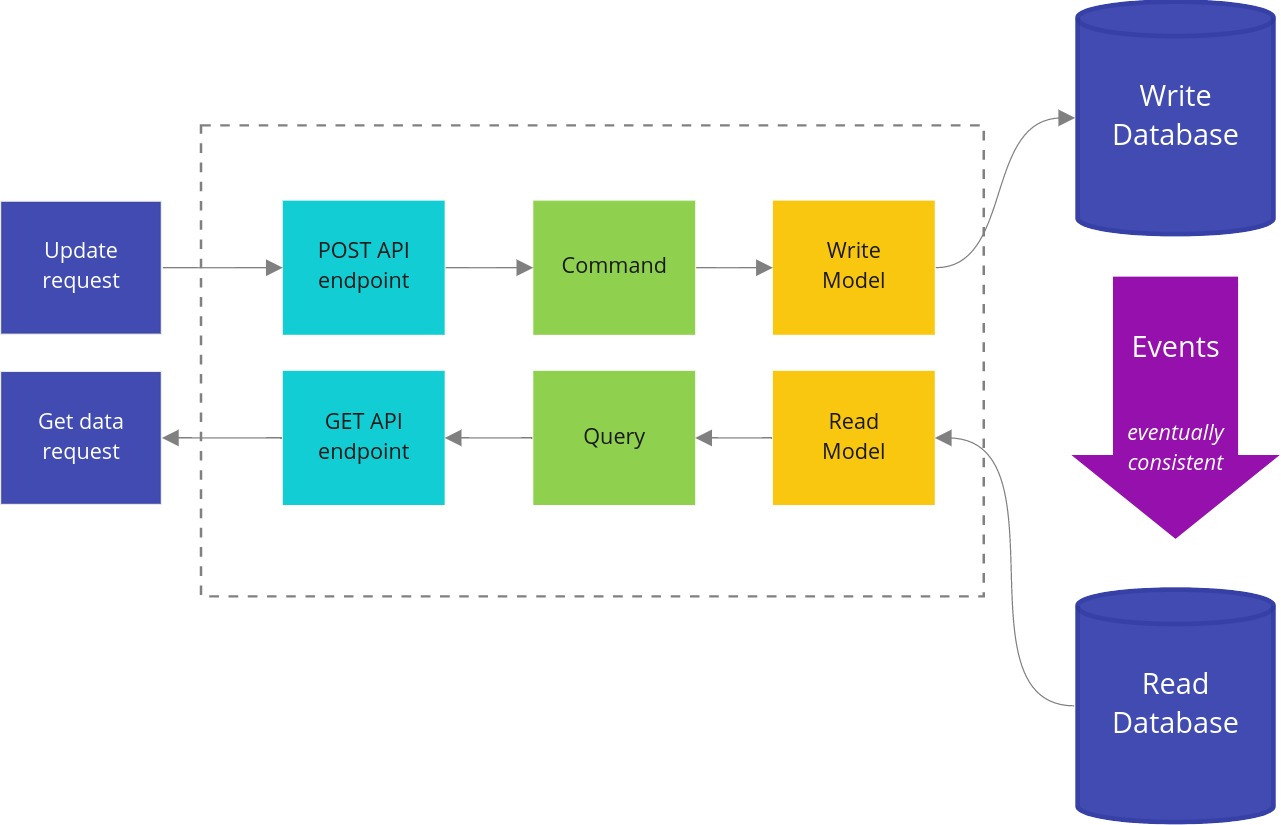
\includegraphics[width=0.7\linewidth]{img/cqrs}
		\caption{Principle of CQRS}
		\label{fig:cqrs}
	\end{figure}
	
	
	All Commands are validated inside the handler and after that generate Events, which are both saved to Event store and sent via Event bus using NATS\footnote{\url{https://nats.io/}}. These events are then listened for and handled by any systems which manage them. Thanks to storing the Events in Event store, the systems, which are not online during the Event generation can then load them from Event store, thus ensuring eventual consistency (see \ref{sec:data-consistency}).	
	
	\begin{figure}
		\centering
		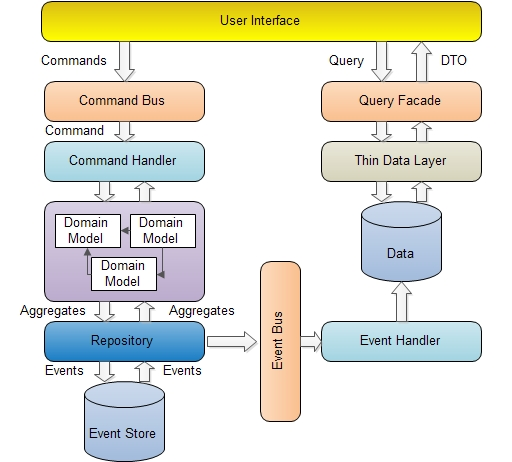
\includegraphics[width=0.7\linewidth]{img/cqrs-event_sourcing}
		\caption{Event sourcing}
		\label{fig:cqrs-eventsourcing}
	\end{figure}
	

\section{How to use}
	The complete application is self-contained and thanks to using Docker\footnote{\url{https://www.docker.com/}} containers, it is easy to run using Docker compose\footnote{\url{https://docs.docker.com/compose/}}. For simplicity, one can use the prepared \texttt{make dev} command, which start all services.
	
	

\section{API documentation}\label{sec:api-documentation}
	The API documentation can be generated using the \texttt{make docs} or \texttt{make run-docs} commands. This will generate Swagger\footnote{\url{https://swagger.io/}} documentation from the code and the latter will also start a small HTTP server with GUI.

\section{Conclusion}
	The implemented project is a slightly cut-down version of the proposed solution due to technical difficulties few days before deadline. It however still implements CQRS pattern with event sourcing and eventual consistency making it highly scalable and consistent.

	
%\newpage
%\nocite{*}
%\bibliography{references}
\end{document}